\documentclass{beamer}
\usepackage[ngerman]{babel}
\usepackage[utf8]{inputenc}
\usepackage{amsmath}
\usepackage{amsthm}
\usepackage{siunitx}
\usepackage{graphicx}
\usepackage{pgfplots}
\sisetup{locale = DE}
% Lade Beamer Stile
\usepackage{beamerthemesplit}
\usepackage{tcolorbox}
\usetheme{Rochester}
\usecolortheme{crane}


\title{1. Unterrichtseinheit zur Dynamik}
\subtitle{Drehmoment und Hebel}
\author{Heiko Schröter}
\date{\today}

\setbeamertemplate{enumerate item}{\alph{enumi})}

\begin{document}

\frame{\titlepage}

\frame
{
  \frametitle{Ziele für die heutige Unterrichtseinheit}
  \textbf{Drehmoment und Hebel}
  \begin{itemize}
	\item Wie ist das Drehmoment definiert?
	\item Welche Bedingung muss erfüllt sein, damit am Hebel Gleichgewicht herrscht?
	\item Wie ermittelt man den Hebelarm bei Kräften, die unter einem Winkel $\alpha$ am Hebel angreifen?
	\item Was sind Beispiele für technische Anwendungen des Hebels?
	\item Beispiele für Berechnungen mit Drehmomenten und Hebelarmen?
  \end{itemize}
}

\frame[allowframebreaks]
{
  \frametitle{Dynamik}
Die Wirkung einer Kraft auf einen drehbar gelagerten Körper hängt von der Wirkungslinie der Kraft ab. Geht die Wirkungslinie durch den Drehpunkt, so bleibt der Körper in Ruhe. Trifft die Wirkungslinie nicht den Drehpunkt, dann wird der Körper in Drehung versetzt.
    \begin{figure}
	  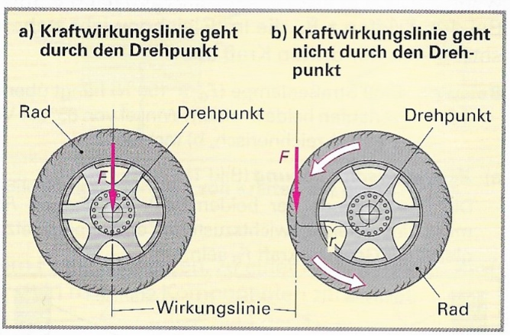
\includegraphics[width=0.5\textwidth]{Drehmoment.png}
	  \vspace{-3mm}
	  \caption{Wirkung einer Kraft auf einen drehbar gelagerten Körper}
   \end{figure}
   \newpage
Die Stärke der Drehwirkung hängt von der Kraft $F$ und dem senkrechten Abstand $r$ Hebelarm) der Wirkungslinie zum Drehpunkt ab. Diese Größe nennt man \textbf{Drehmoment $M$}.
    \begin{figure}
	  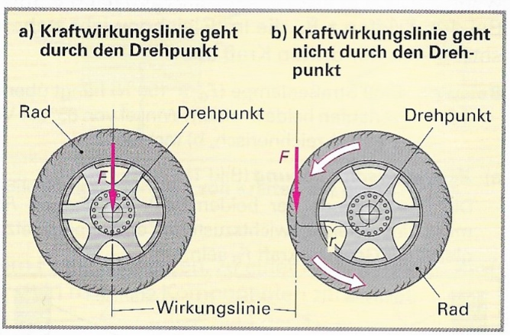
\includegraphics[width=0.5\textwidth]{Drehmoment.png}
	  \vspace{-3mm}
	  \caption{Wirkung einer Kraft auf einen drehbar gelagerten Körper}
   \end{figure}
}

\frame[allowframebreaks]
{
  \frametitle{Definition vom Drehmoment}
  \begin{block}{Drehmoment}
	\begin{align}
	M=F\cdot r
	\end{align}
  \end{block}
  \begin{itemize}
  \item Die Einheit vom Drehmoment ist $\si{\newton\meter}$ und das Formelzeichen ist $M$.
  $[M]=[F]\cdot[r]=\si{\newton\meter}$
  \item Wirkt z.B. eine Kraft von $\SI{350}{\newton}$ im Abstand von $\SI{0.15}{\meter}$ zum Drehpunkt, so beträgt das Drehmoment $M=F\cdot r=\SI{350}{\newton}\cdot\SI{0.15}{\meter}=\SI{52.5}{\newton\meter}$. 
  \end{itemize}
}

\frame[allowframebreaks]
{
  \frametitle{Hebel und Drehmomentengleichgewicht}
Ein Hebel ist ein starrer Körper, der um eine feste Achse drehbar gelagert ist. Je nach Lage des Drehpunktes unterscheidet man in einseitige, zweiseitige sowie Winkelhebel. Am Hebel angreifende Kräfte versuchen ihn entweder links oder rechts herum zu drehen. Der Hebel bleibt in Ruhe (Gleichgewicht), wenn die linksdrehende Wirkung genau so groß ist wie die rechtsdrehende Wirkung. 
  \begin{block}{Hebelgesetz}
Ein Hebel befindet sich im Gleichgewicht, wenn das Produkt aus Last $F_{L}$ und Lastarm $r_{L}$ gleich dem Produkt aus Kraft $F_{F}$ und Kraftarm $r_{F}$ ist.	
	\begin{align}
	F_{L}\cdot r_{L}=F_{F}\cdot r_{F}
	\end{align} 
  \end{block}
    \begin{block}{Beim Gleichgewicht}
An einem Hebel herrscht Gleichgewicht, wenn die Summe der rechtsdrehenden Drehmomente gleich der Summe der linksdrehenden Drehmomente ist:	
	\begin{align}
	\Sigma M_{r}=\Sigma M_{l}\\
	\Sigma \overrightarrow{M}=0
	\end{align} 
  \end{block}  
    \begin{figure}
	  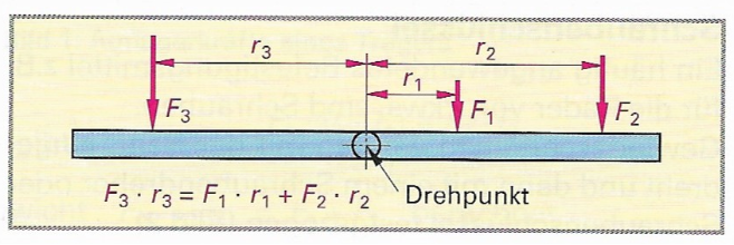
\includegraphics[width=0.65\textwidth]{Gleichgewicht.png}
	  \vspace{-3mm}
	  %\caption{Wirkung einer Kraft auf einen drehbar gelagerten Körper}
   \end{figure}  
}

\frame{
  \frametitle{Der wirksame Kraftarm}
    \begin{figure}
	  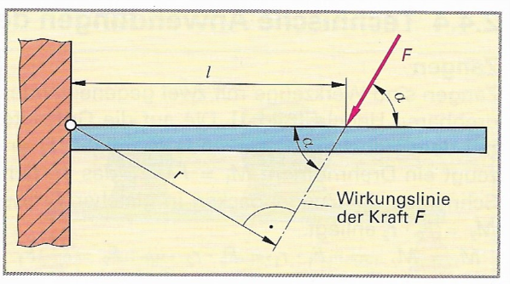
\includegraphics[width=0.5\textwidth]{Kraftarm.png}
	  \vspace{-3mm}
	  \caption{Wirksamer Kraftarm $r$ des Drehmoments}
   \end{figure}    
  \begin{block}{}
  Der wirksame Kraftarm $r$ ist der senkrechte Abstand vom Drehpunkt zur Wirkungslinie der Kraft $F$. Für eine Kraft, die wie im Bild unter einem Winkel $\alpha$ am Hebel angreift, gilt:
	\begin{align}
	M=F\cdot r = F\cdot l\cdot \sin\alpha
	\end{align}  
  \end{block}

}

\frame[allowframebreaks]
{
  \frametitle{Technische Anwendungen des Hebels}
    \begin{figure}
	  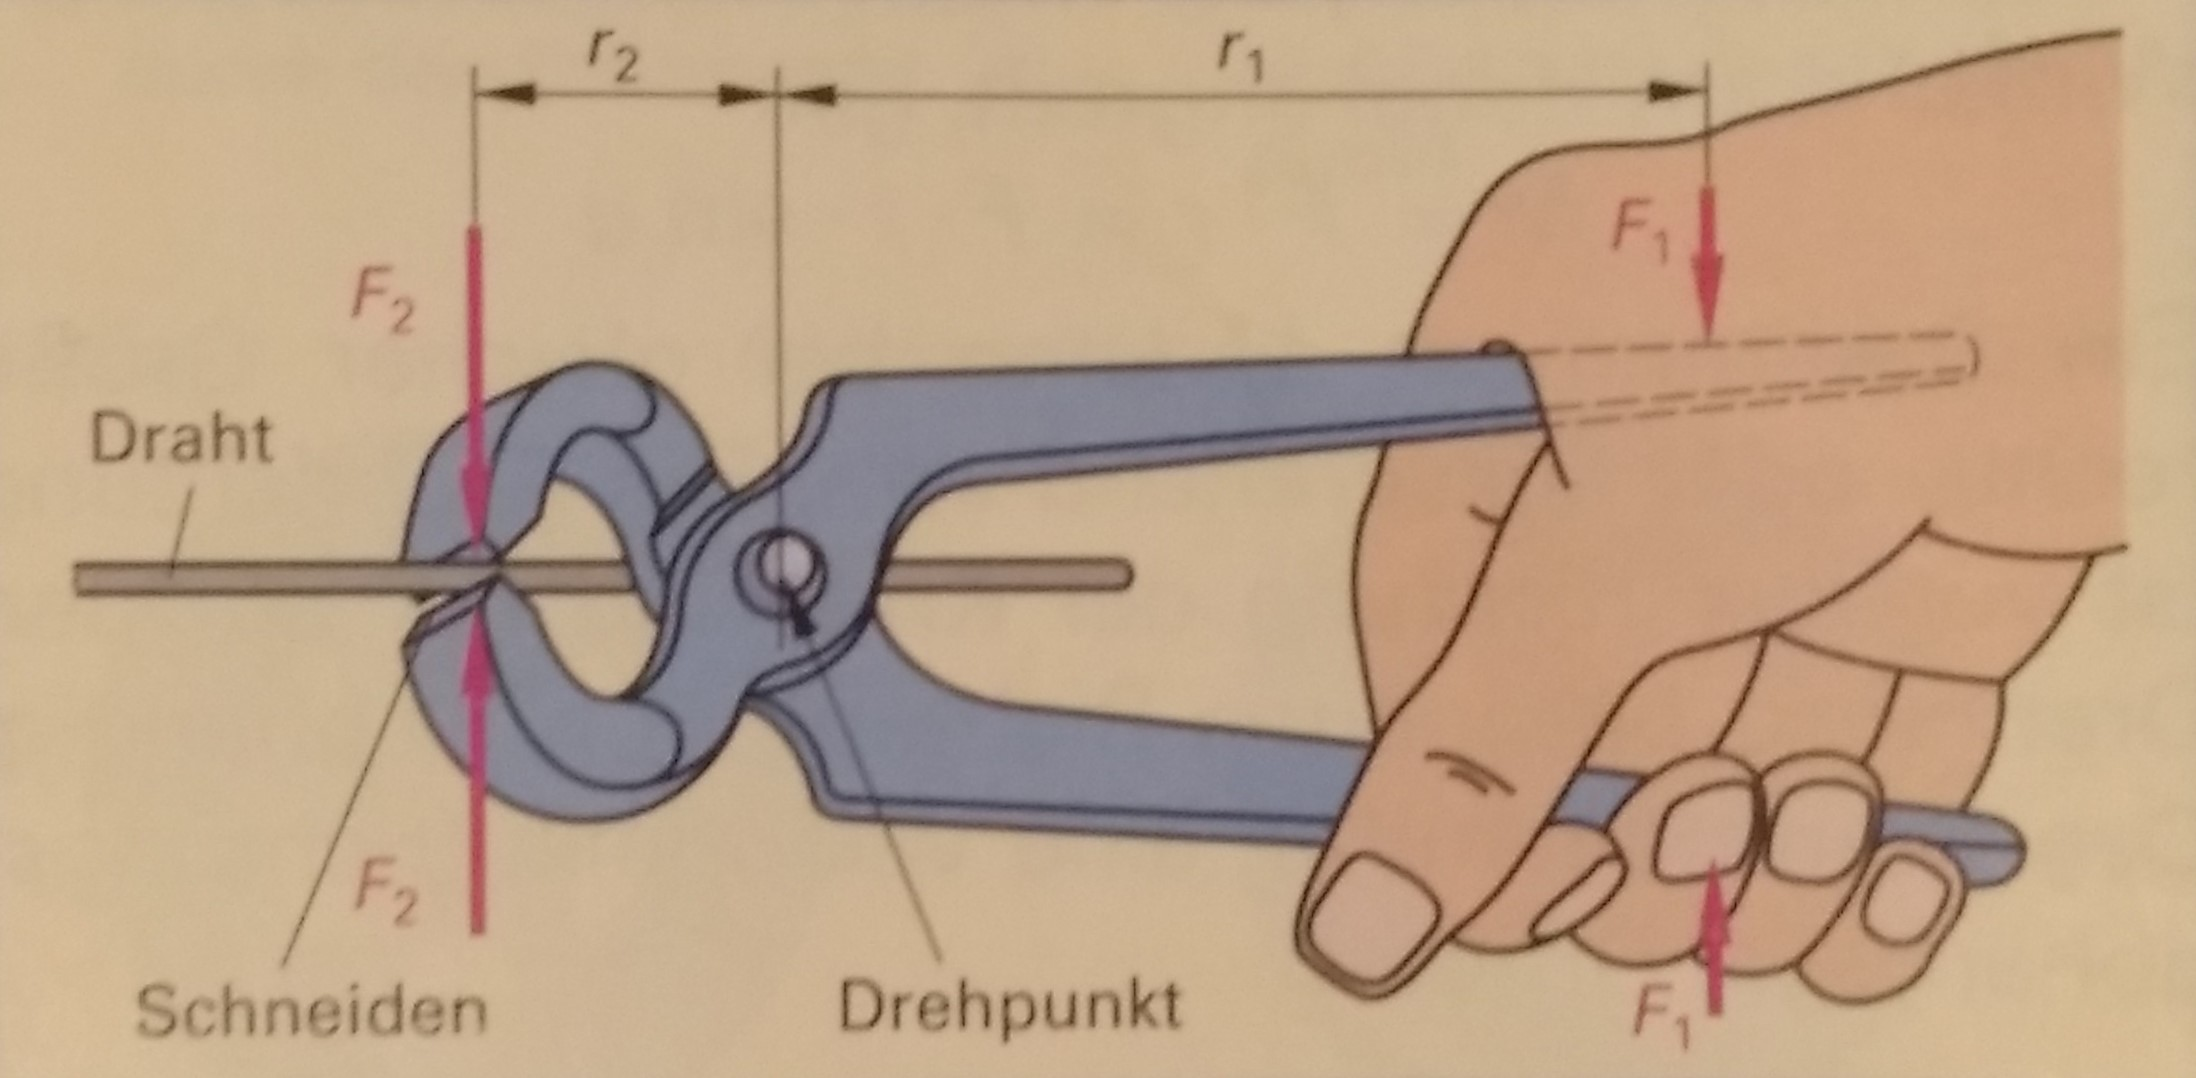
\includegraphics[width=0.8\textwidth]{Zange}
	  \caption{Hebel einer Kneifzange}
	  \newpage
	  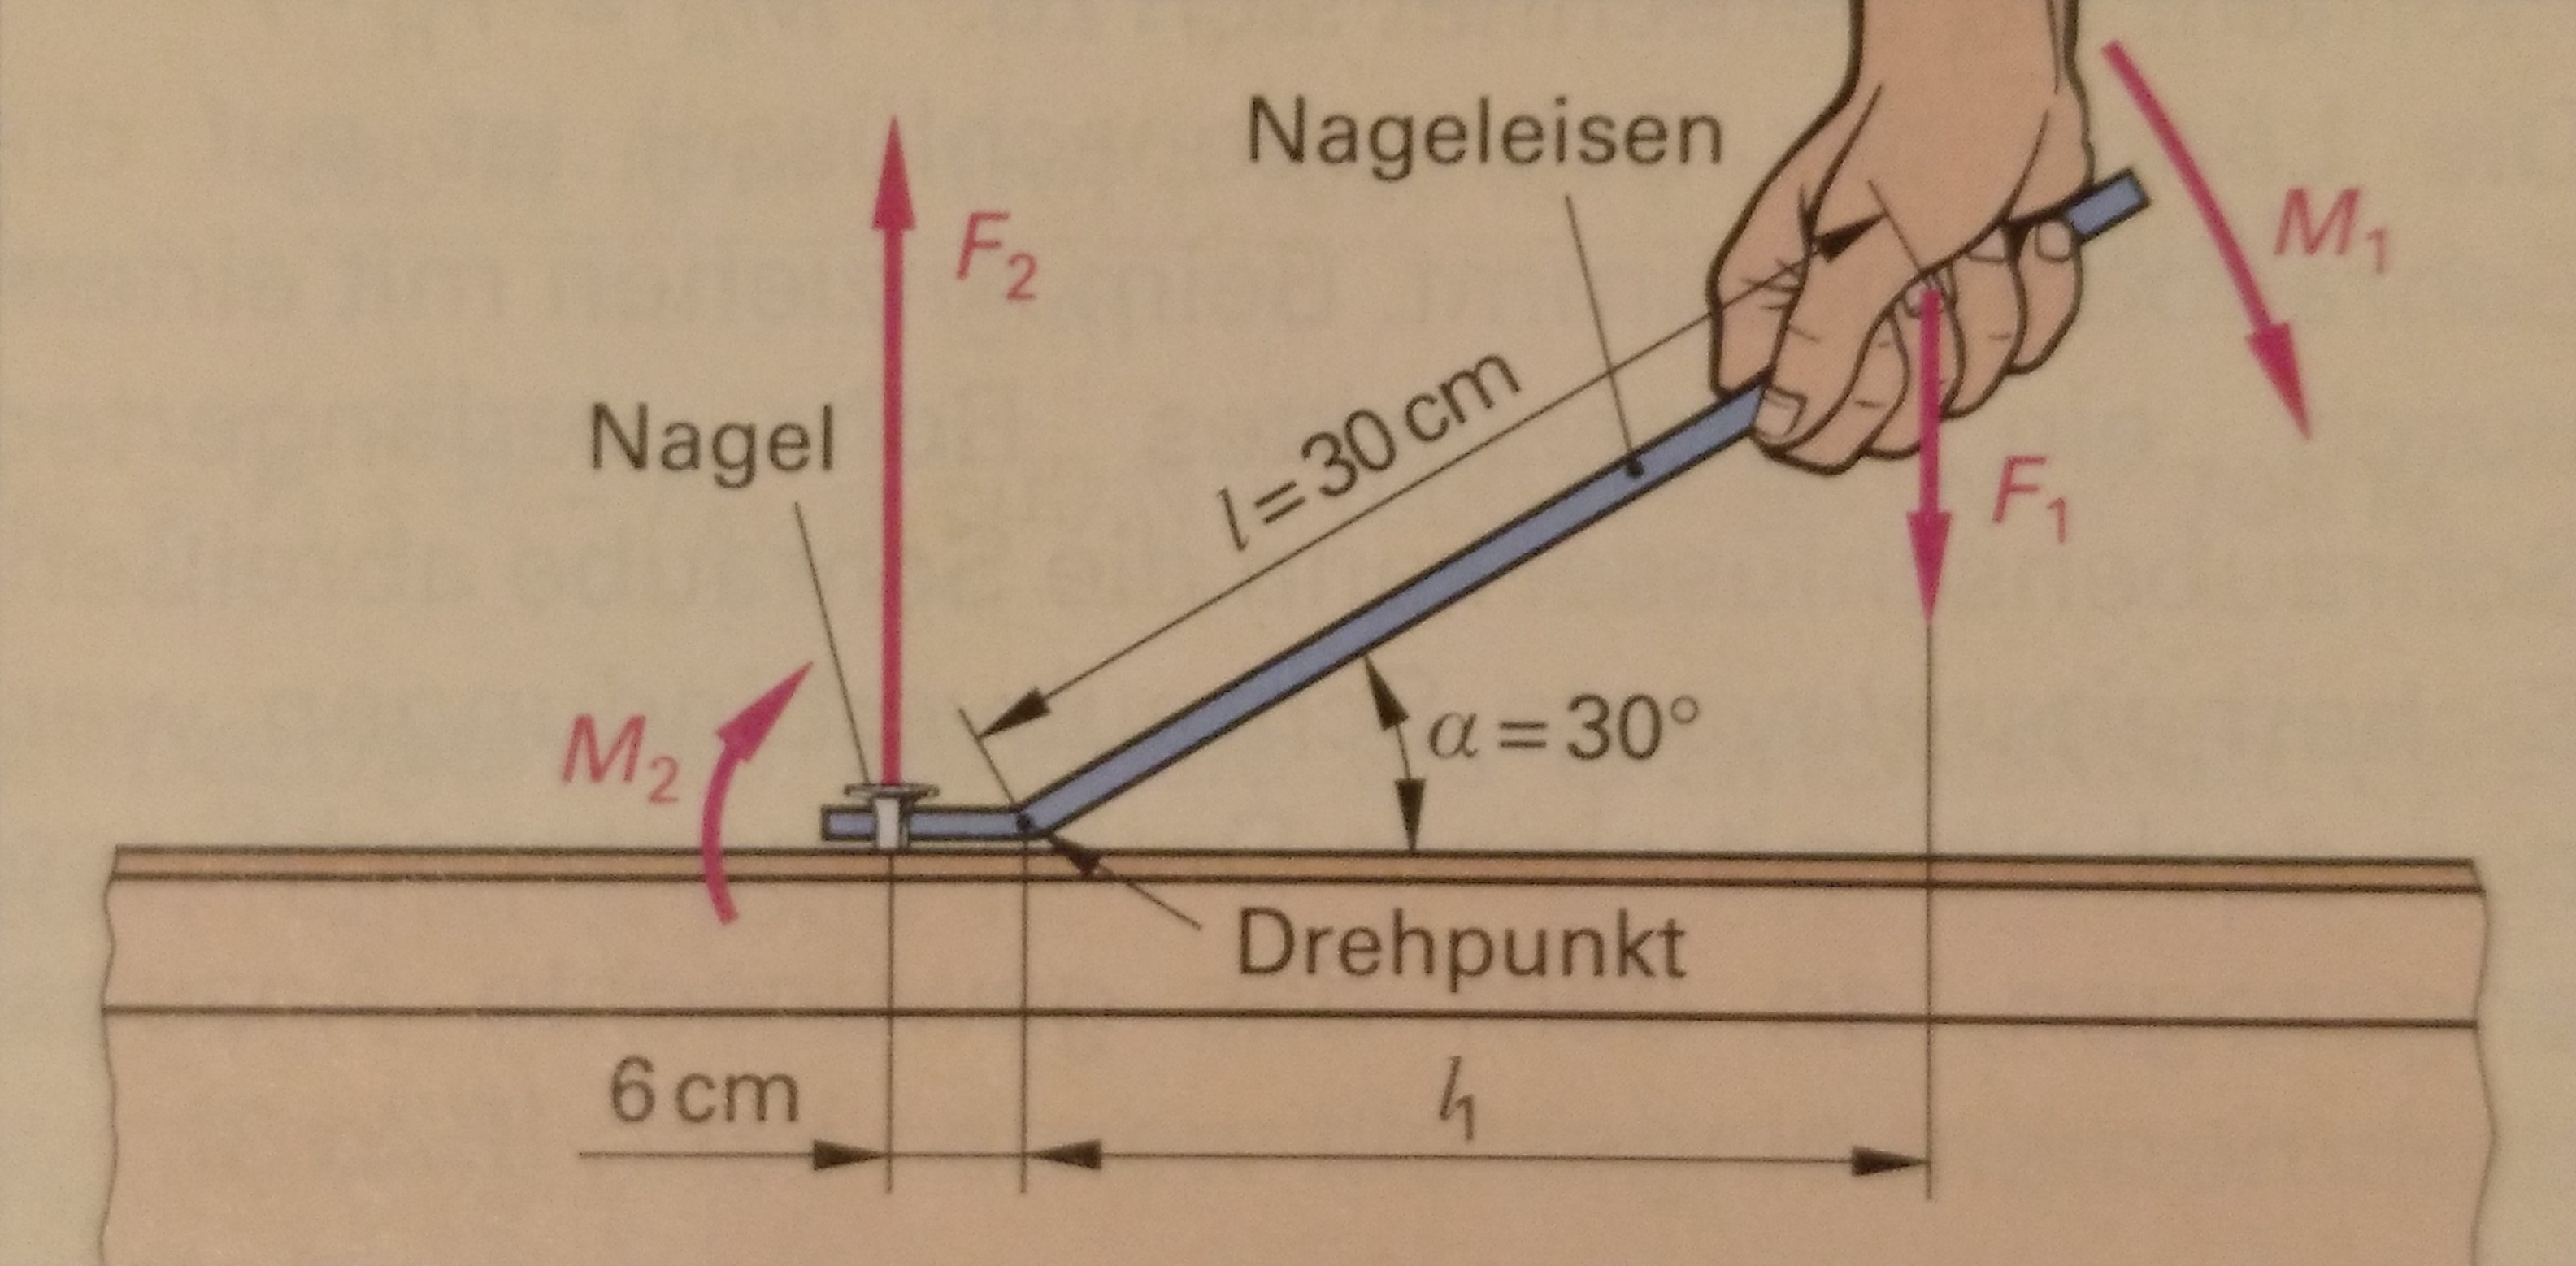
\includegraphics[width=0.8\textwidth]{Nageleisen.jpg}
	  \caption{Ziehen von Nägeln mit dem Nageleisen}
	  \newpage
	  \includegraphics[width=0.8\textwidth]{Schraubenschlüssel.jpg}
	  \caption{Hebelwirkung beim Anziehen einer Schraube}
	  \newpage
	  \includegraphics[width=0.8\textwidth]{Drehmomentschlüssel.jpg}
	  \caption{Drehmomentenschlüssel}
	  \newpage
	  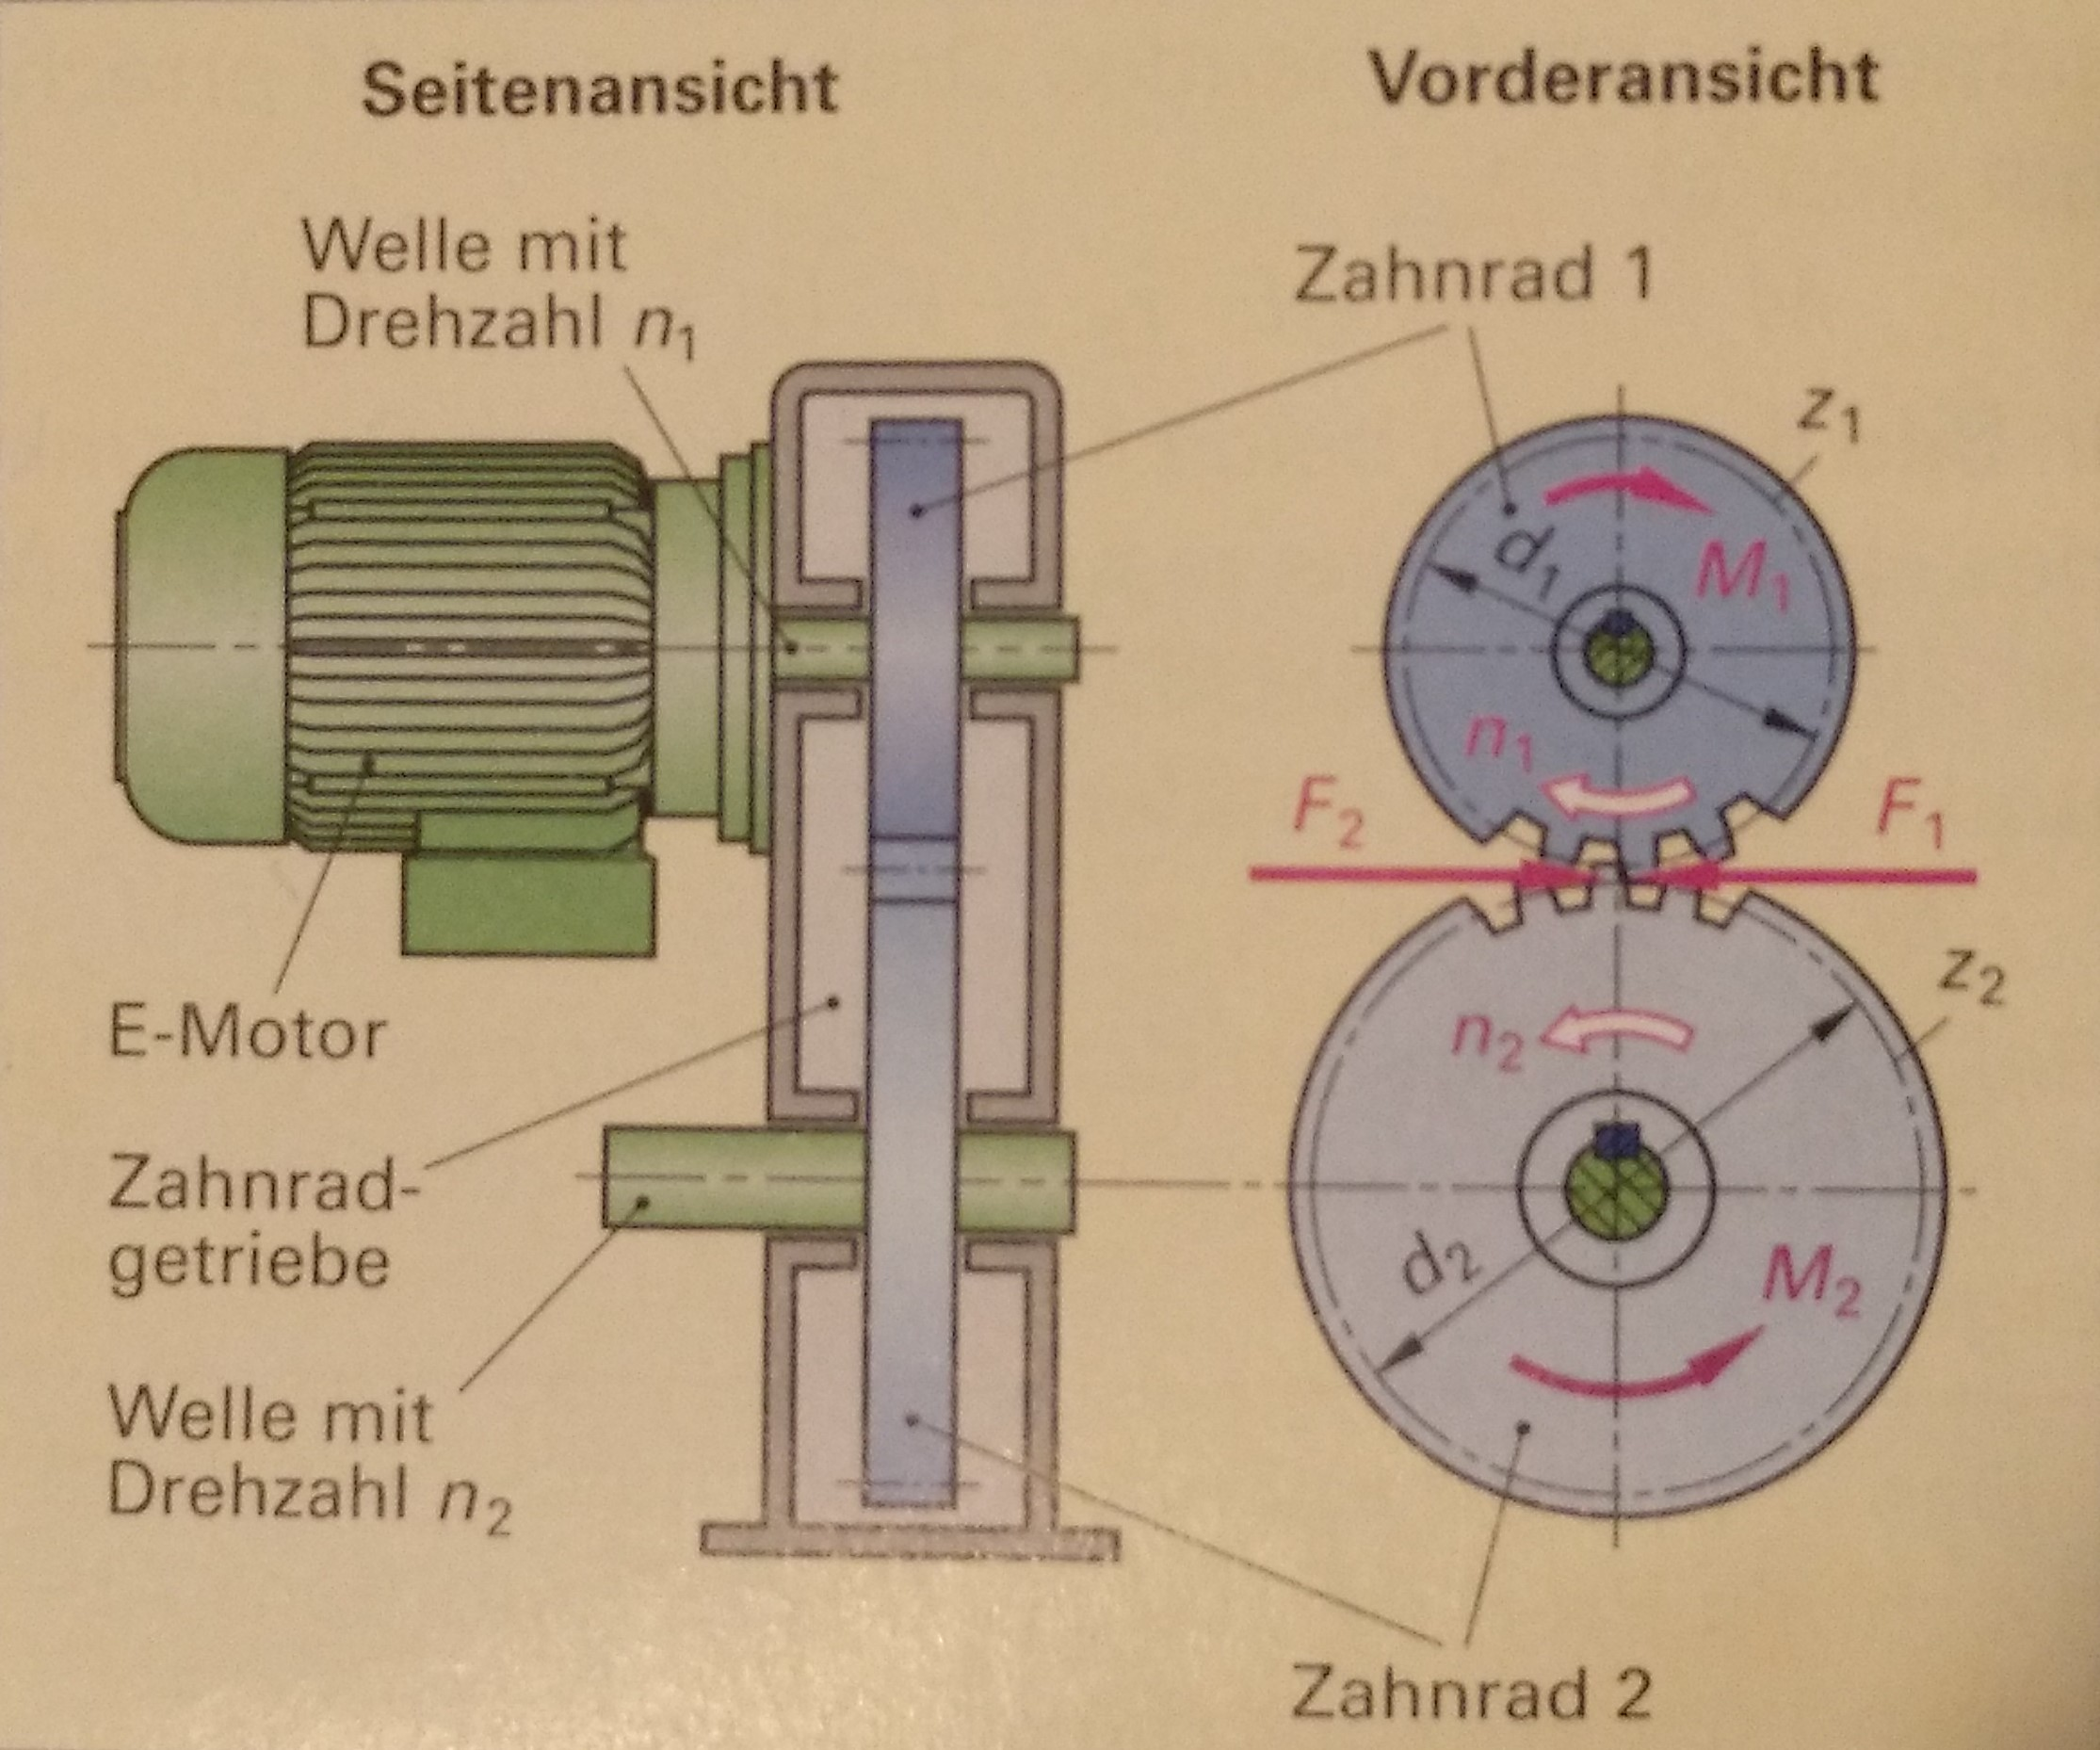
\includegraphics[width=0.7\textwidth]{Zahnradgetriebe.jpg}
	  \caption{Hebelwirkung beim Zahnradgetriebe}	  	  	  
    \end{figure}
}

\frame
{
\frametitle{Übung - \textbf{Drehmoment} und Hebel}
\begin{enumerate}
\item[1.] Berechnen Sie das Moment beim Anziehen einer Schraube mit einer Kraft von $\SI{120}{\newton}$ bei einem wirksamen Hebelarm von $\SI{180}{\milli\meter}$.
\item[2.] Eine Schraube $M20$ darf höchstens mit einem Moment von $\SI{145}{\newton\meter}$ angezogen werden. Berechnen Sie die zulässige Kraft bei einer Schlüssellänge (Hebellänge) von $\SI{220}{\milli\meter}$, wenn der Winkel zwischen Kraftrichtung und Hebel $\SI{80}{\degree}$ beträgt.
\item[3.] Auf eine Antenne wirkt eine Windkraft von $\SI{200}{\newton}$. Das zulässige Moment an der Einspannstelle beträgt $\SI{680}{\newton\meter}$. In welchem Abstand von der Einspannstelle darf die Antenne höchstens montiert werden?
\item[4.] Ein $\SI{10}{\tonne}$-Kran hat ein zulässiges Lastmoment von $\SI{2}{\mega\newton\meter}$. Berechnen Sie die maximale Ausladung.
\end{enumerate}
}

\frame[allowframebreaks]
{
\frametitle{Übung - Drehmoment und \textbf{Hebel}}
\begin{enumerate}
\item[5.] Bei der Ventilsteuerung eines Kraftfahrzeuges greift der Steuernocken (siehe Abbildung) am Kipphebel an. In welchem Abstand $r_{2}$ vom Drehpunkt des Kipphebels muss der Steuernocken angebracht werden, wenn die Kraft des Nockens $\SI{600}{\newton}$ und die Öffnungskraft der Ventilfeder $\SI{480}{\newton}$ betragen?
    \begin{figure}
	  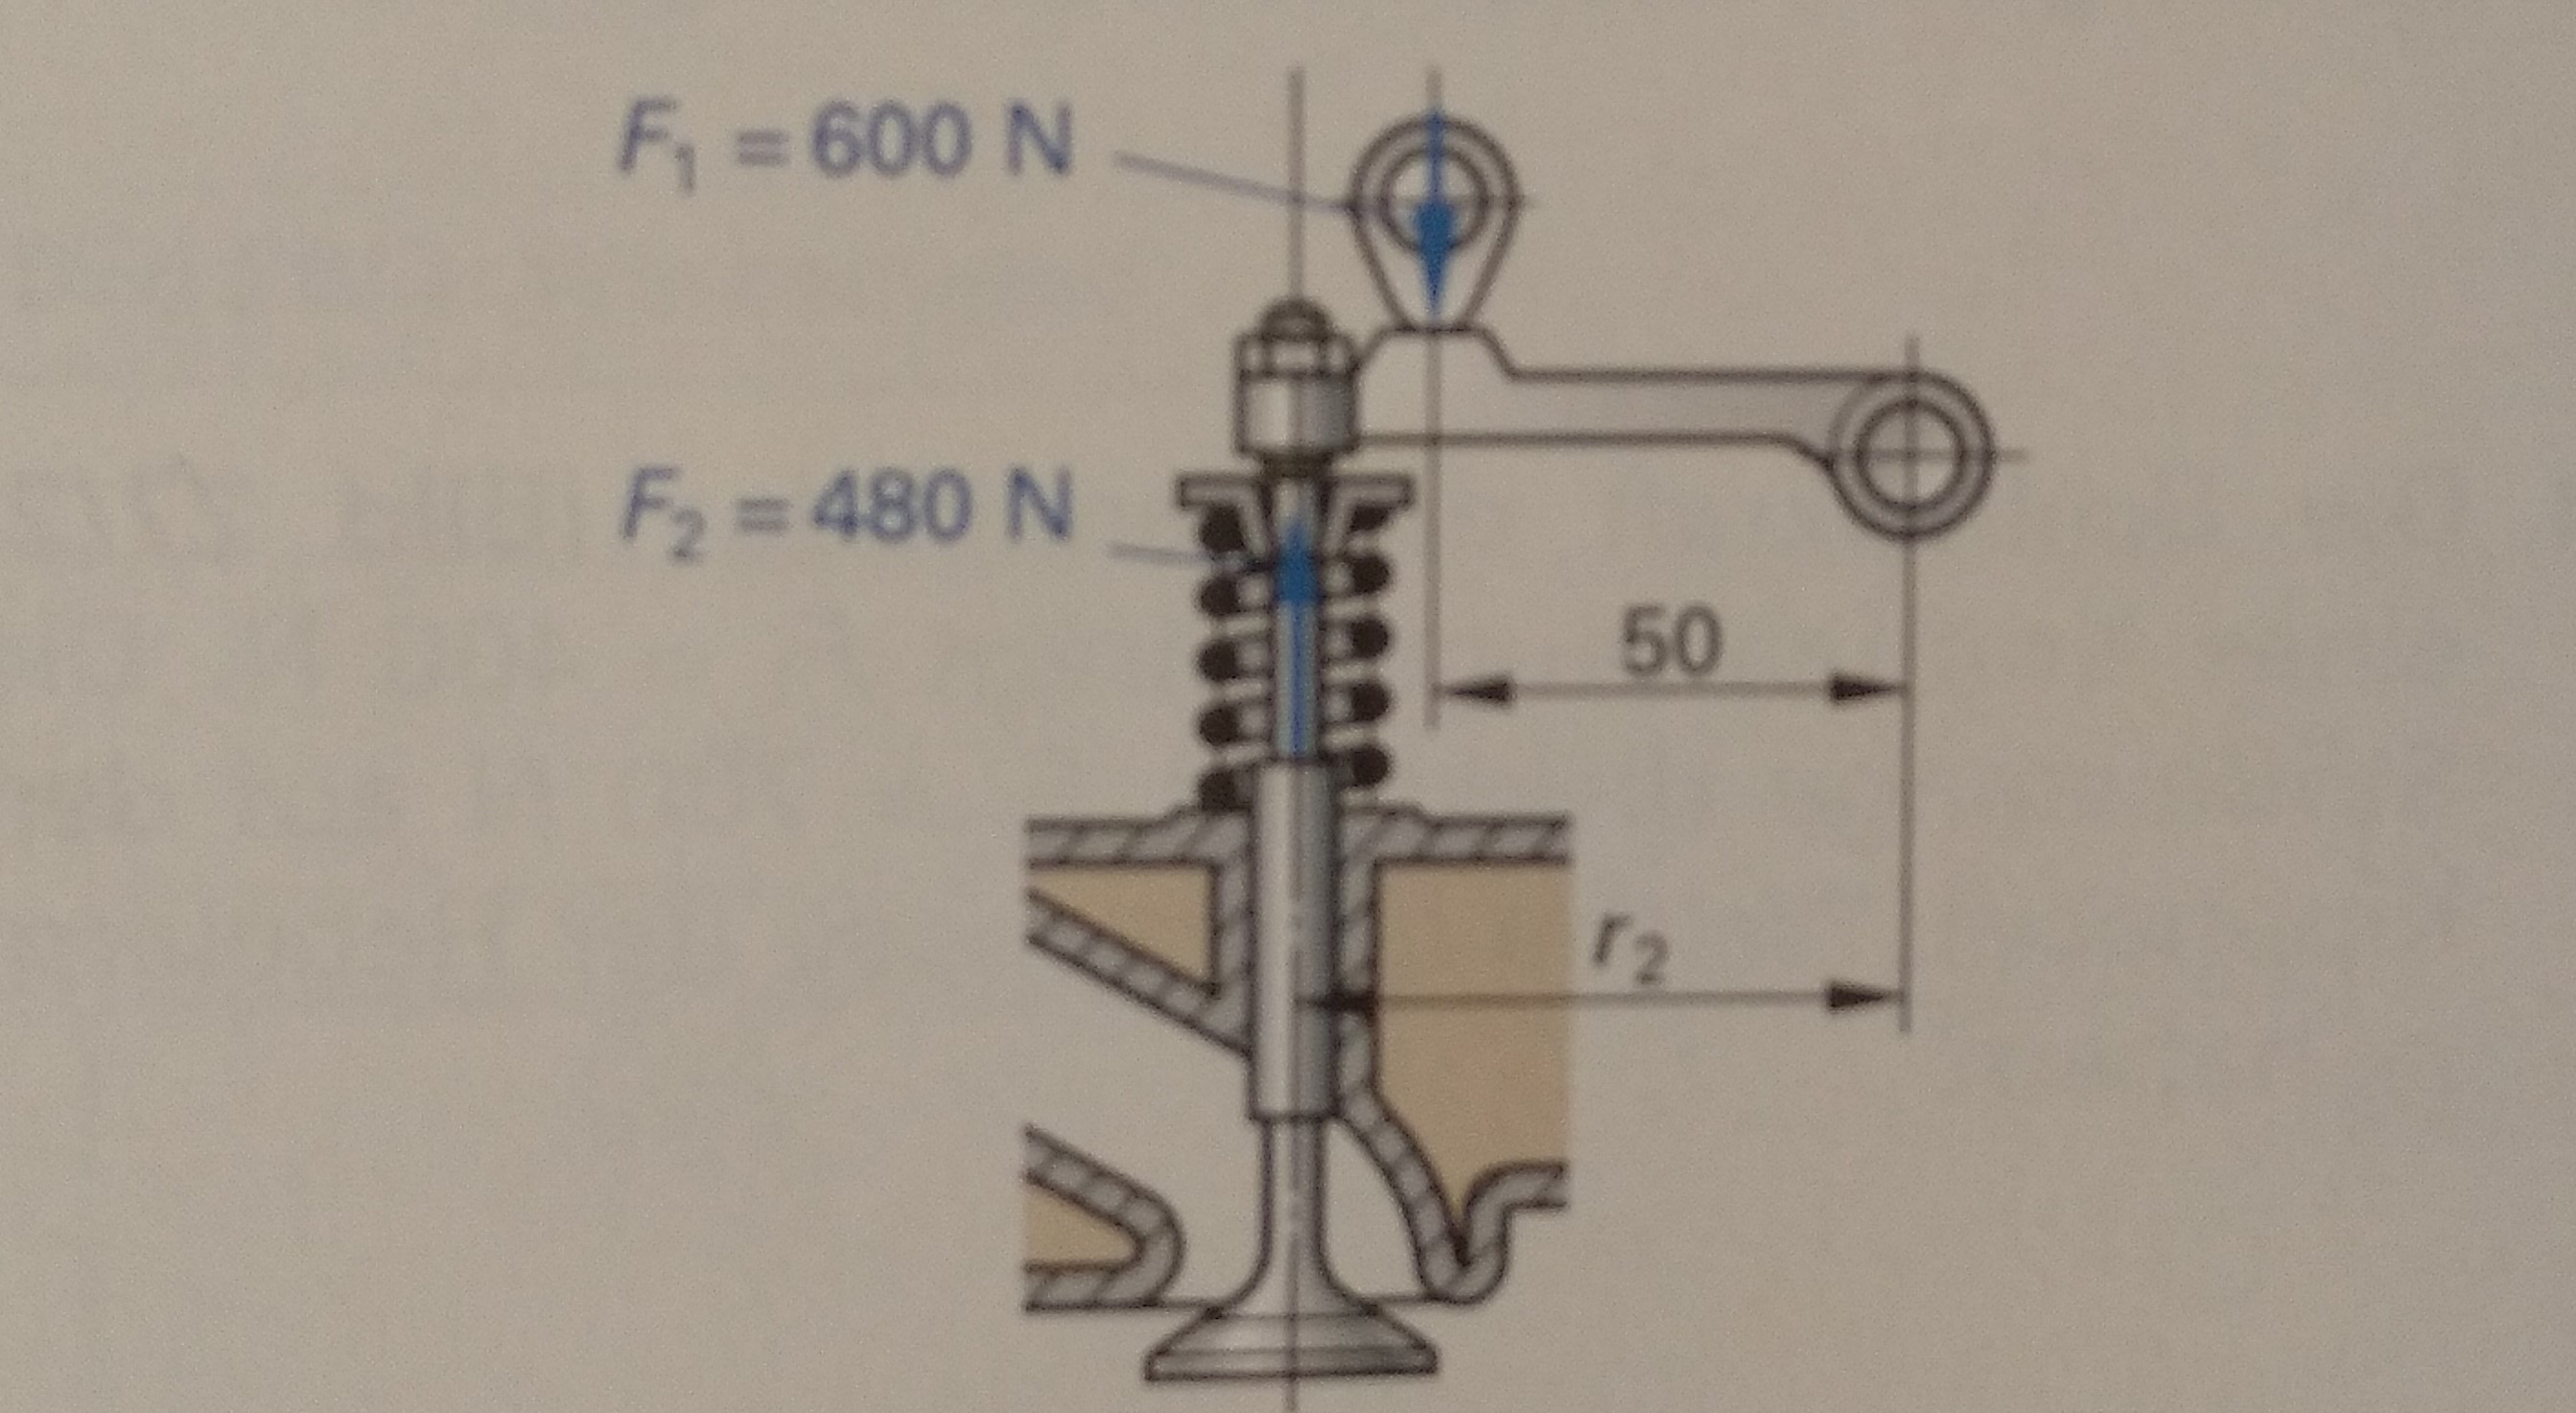
\includegraphics[width=0.6\textwidth]{Ventilsteuerung.jpg}
	  \vspace{-3mm}
	  \caption{Ventilsteuerung}
   \end{figure}
\item[6.] Die Fußkraft an einem Bremspedal beträgt $F_{1}=\SI{300}{\newton}$. Der Winkel zwischen $\overrightarrow{F_{2}}$ und dem Hebelarm beträgt $\SI{45}{\degree}$. Berechnen Sie die Kraft $F_{2}$ der Kolbenstange (siehe Abbildung).
    \begin{figure}
	  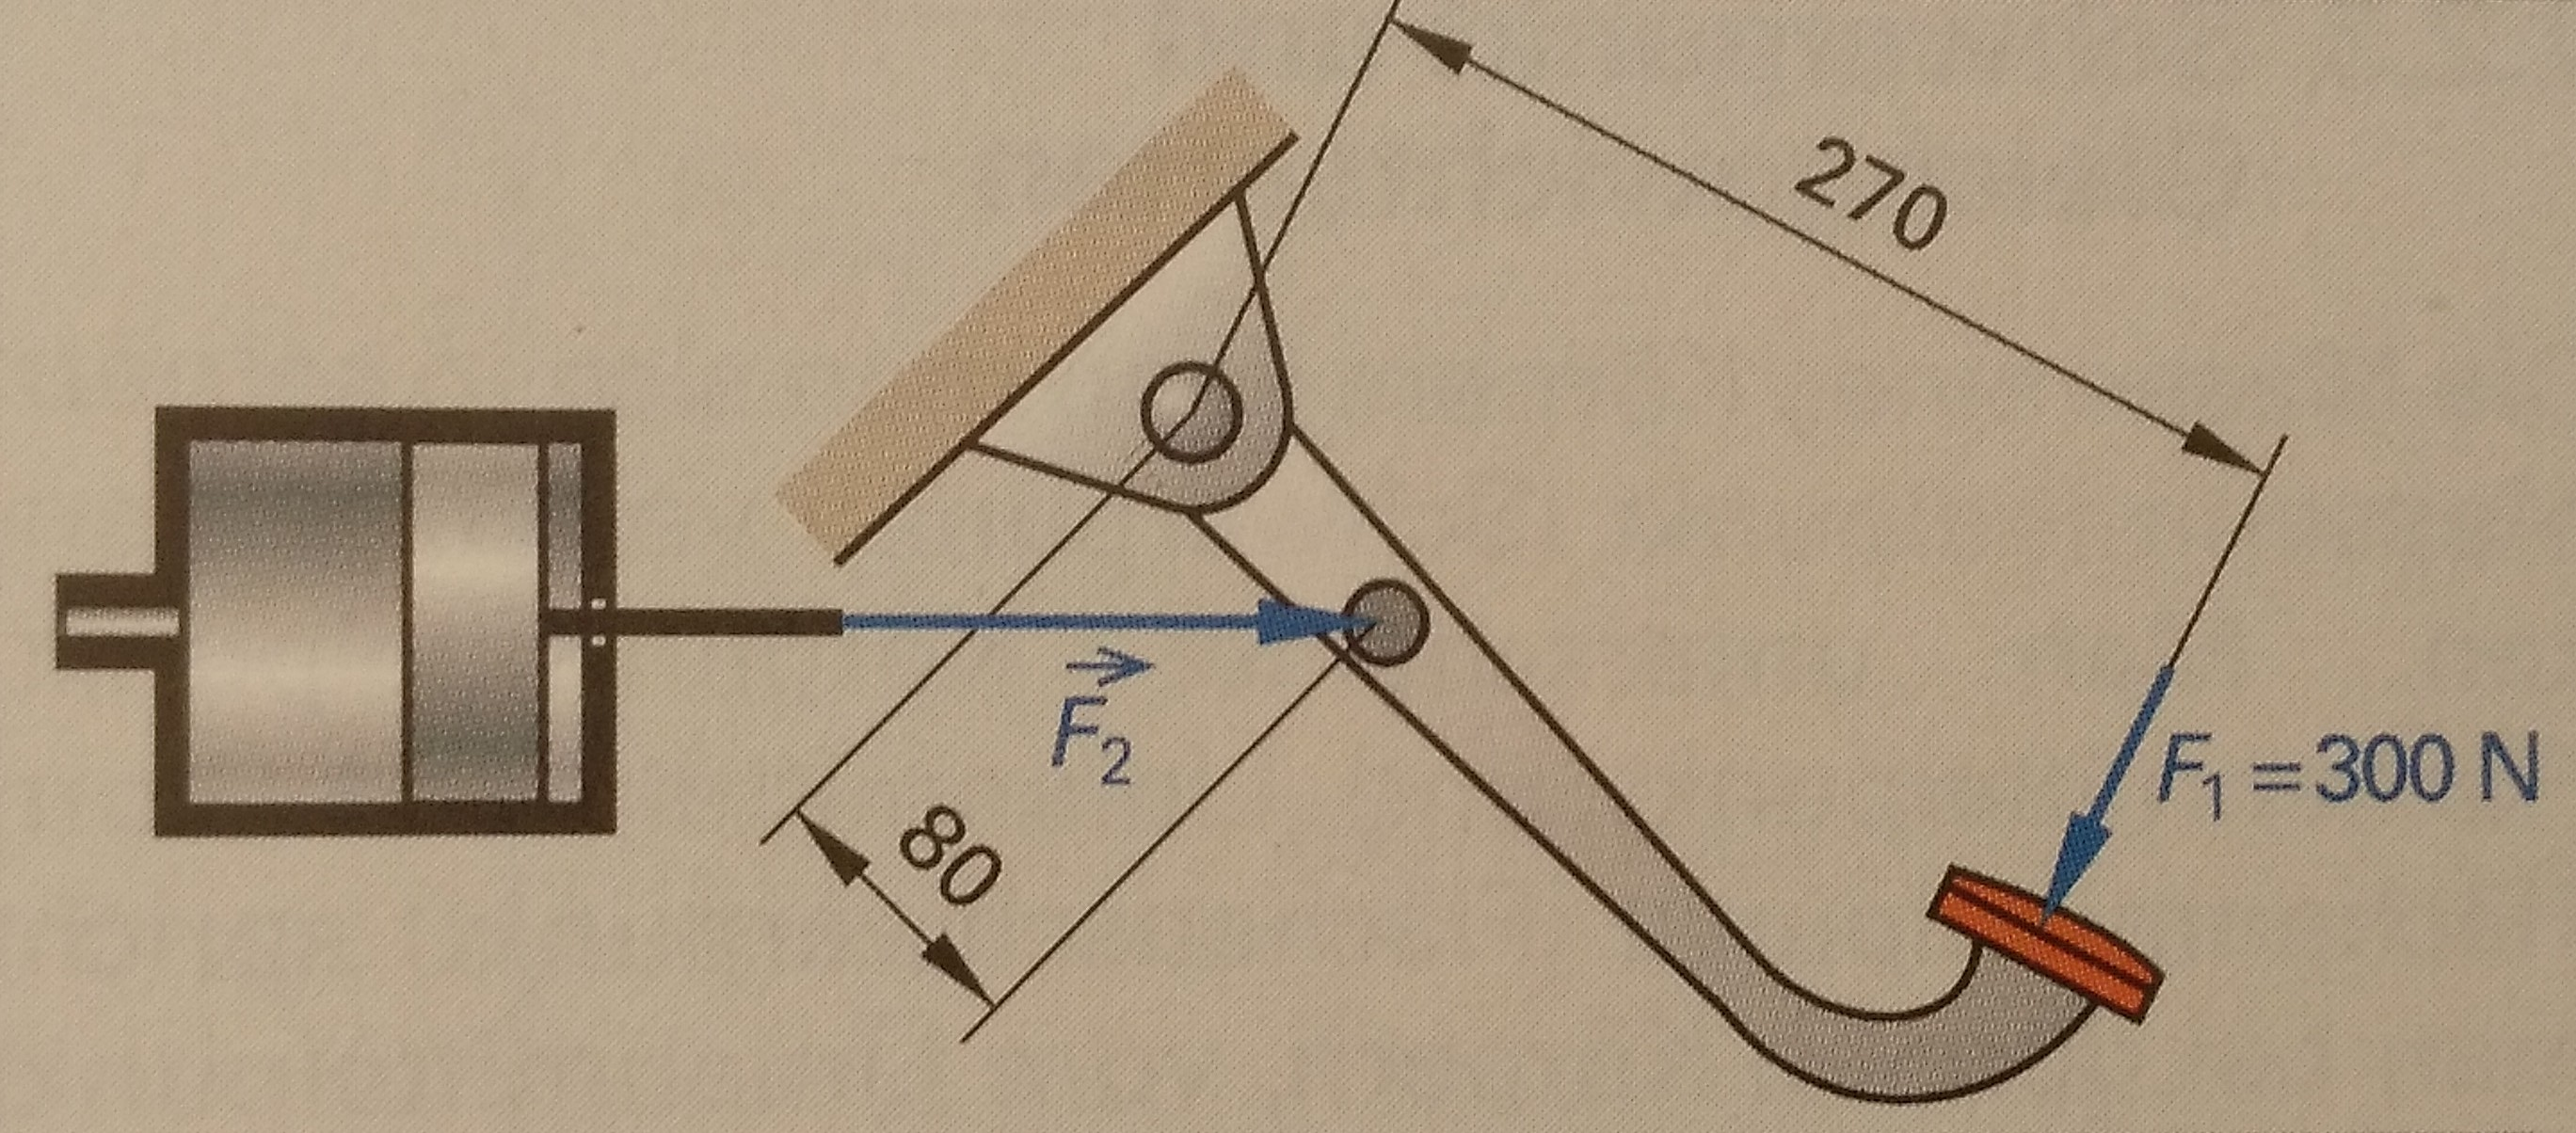
\includegraphics[width=0.6\textwidth]{Bremspedal.jpg}
	  \vspace{-3mm}
	  \caption{Bremspedal}
   \end{figure}
\end{enumerate}
}

\end{document}
